\documentclass{article}
\usepackage{graphicx}
\usepackage{hyperref}
\usepackage[a4paper, margin=1in]{geometry}
\usepackage{breakcites}
\usepackage{subcaption}
\usepackage{multicol}
\usepackage{booktabs}
\usepackage{longtable}
\usepackage{authblk}

\begin{document}

\title{Mapping Africa's Natural Safety Nets: Where Should Conservation Efforts Be Targeted to Sustain Ecosystem Services for Climate Change Resilience?}

\author[1,2,*]{Cooper, Matthew}

\affil[1]{T.H. Chan School of Public Health, Harvard University}
\affil[2]{Department of Geographical Sciences, University of Maryland College Park}
\affil[*]{Corresponding Author: mcooper@hsph.harvard.edu}

\maketitle
\begin{abstract}

In Africa, where millions of households depend on rainfed agriculture to produce food for their own consumption, climate change is a major threat to food security.  A large literature suggests that natural areas can be an asset in the face of climate change by shielding cropland from the effects of droughts and heat waves, while also providing wild foods when yields are low.  However, much of the work focusing on the safety net provided by natural and uncultivated land has been conducted in highly localized and site-specific case studies which often rely on hypothetical or retrospective analyses.  To date, there has been little empirical and spatially explicit work on which areas provide the most benefit to local food security.  In this study, we combine data on nutrition outcomes from 221,225 children in agrarian communities across 32 African countries with historical observations of land cover and climate shocks to test the hypothesis that uncultivated land can act as a safety net in certain contexts.  We find that in woodland, semi-humid agro-ecological zones in Africa, children in areas with more uncultivated land cover are less drought affected than those in areas with more agricultural land cover.  Finally, we map where conservation interventions could have the largest impact on improving nutritional resilience to future droughts, and compare our results to priority areas for conserving biodiversity to identify African landscapes where conservation could provide multiple benefits.

\end{abstract}

\section{Introduction}

Currently, an estimated 58.8 million African children, representing nearly one third of the continent's under-5 population, suffer from chronic undernutrition \cite{unicef2019}.  While progress has been made in the past several decades to improve nutrition and food security outcomes, climate change threatens to stall or even reverse current trends \cite{FAO2018}.  As climate change continues, the frequency and intensity of meteorological extremes will affect food production, ultimately harming food security and nutrition for many vulnerable communities.  Africa is particularly vulnerable to these changes, as an estimated 95\% of agriculture is rainfed \cite{Wani2009} and about 65\% of households produce food for their own consumption \cite{Runge2004}.

One factor that can play a major role in fostering food systems that are resilient to climate shocks is the presence of ecosystem services provided by natural, uncultivated areas \cite{Reed2016, Pascual2017, Daily2008}.  These area provide a suite of regulating services that can buffer agricultural yields from the effects of shocks.  For example, natural vegetation can provide shade and cooler temperatures during heat waves, absorb water and protect against erosion during floods, as well as retain soil moisture during droughts \cite{Siriri2013, Lott2009}.  Furthermore, natural areas can provide habitat for pollinators and species that regulate pest outbreaks \cite{Karp2013}.  Beyond regulating services, uncultivated land provides provisioning services in the form of wild foods and other inedible products that can support local incomes and food security when agricultural output is low \cite{friant2019life, morgan2020secret, powell2015improving, Assogbadjo2012}.

A great deal of literature has focused on the benefit that ecosystem services can provide, although much of this work has relied on studies that are site specific.  For example, detailed work conducted in case studies across Africa have found instances of ecosystem services improving nutrition \cite{Golden2011}, regulating crop pests \cite{Girma2000}, improving yields through pollination \cite{Gemmill-Herren2008, Munyuli2012}, and improving soil nutrient quality \cite{Sileshi2012, Boffa2000, Siriri2009}.  Some work that is particularly relevant to climate resilience has found that natural land cover can improve soil water storage \cite{Siriri2013, Lott2009}, but nevertheless few empirical studies have observed how ecosystem services affect human outcomes during climate shocks.  Rather, most studies that focus on ecosystems as a form of climate resilience use surveys that ask respondents if they would rely on ecosystem services in the event of a hypothetical shock \cite{Robledo2012}, with some studies indicating that many people do not think of ecosystem services as an asset that they would rely on during shocks \cite{Wunder2014}.

Building on all these case studies, a growing body of work has drawn on Demographic and Health Surveys from across Africa and the developing world to assess whether the benefits provided by various ecosystem services can be observed at scale.  This work has shown that forest cover is associated with improved dietary diversity \cite{Ickowitz2014, Rasolofoson2018}, that forested watersheds are associated with less diarrheal disease \cite{Herrera2017}, and that protected areas are associated with a number of positive benefits \cite{naidoo2019evaluating}.  However, while these studies have found large-scale associations between environmental variables and positive human outcomes, little work has examined spatial heterogeneities in these associations in order to examine climate resilience or inform conservation priority setting.

While a large body of research attests to the fact that ecosystem services play an important role in food production and nutrition, especially for smallholder farmers, comparatively little work in the field of environmental conservation has been conducted to identify areas where conservation interventions could lead to improved food security and nutrition outcomes.  This is in spite of the fact that the practice of conservation relies heavily on mapping for priority setting - for example, mapping ecosystem services such as carbon sequestration and storage \cite{Kim2016} or water provision \cite{immerzeel2020importance} as well as mapping biodiversity hot spots \cite{holland2012conservation}.  Thus, conducting environmental epidemiology using large, geolocated datasets on human well-being like the DHS could be useful for mapping which natural areas contribute the most to human well-being and further catalyze conservation investment, as well as identify locations where conservation interventions could lead to synergies between Sustainable Development Goals (SDGs) related to environmental conservation (13 \& 15) and human well-being (1 \& 2), two goals that are often perceived to be in conflict \cite{moore2016improving, mcshane2011hard}.

This paper aims to fill that research gap by examining the benefit that uncultivated land cover provides specifically to nutrition outcomes during droughts.  This study goes beyond testing for broad associations, but also examines how the relationship between climate shocks, natural land cover, and rainfall varies across agro-ecological zones (AEZs) to identify areas where natural land cover provides the greatest benefit to child nutrition outcomes and could inform conservation priority setting.

\section{Theoretical Framework}

\subsection{Land Cover and Ecosystem Services}
The ecosystem services provided by nature are highly varied and operate across different spatial scales.  They are typically classified into provisioning, supporting, regulating, and cultural services \cite{Martinez-Harms2012}, although other typologies exist \cite{Fisher2008}.  A common approach for mapping ecosystem services is to focus on land cover types, especially when primary data is unavailable \cite{Martinez-Harms2012}.  One approach is to analyze each land cover type as providing a ``bundle" of associated ecosystem services \cite{Raudsepp-Hearne2010}.  Thus, in an African context, cultivated land provides food crops as a service, grasslands provide grazing for livestock as well as habitat for pollinators and pest regulation services, while forests provide a variety of wild foods, soil formation, water quality regulation, and non-timber forest products.  This framework is especially useful for analyzing trade-offs: as natural vegetation is cleared to make room for crop production, the increase in food crops necessitates a decrease in habitat for pollinators and wild food species, as well as the regulating services provided by uncultivated land.  Conversely, as agricultural land is abandoned, it stops providing food crops but becomes available again for services such as wild food provision, water quality regulation and erosion protection.  Supporting this framework that uses land cover as proxy for ecosystem services, previous work has shown that natural, uncultivated land is one of the best geographic predictors of whether households in Africa report collecting both wild foods as well as other provisioning ecosystem services \cite{Cooper2018a}.

\subsection{Uncultivated Land and Commons}
The regulating and supporting services provided by uncultivated land, such as soil formation, pollination, and water retention are, by their very nature, beneficial across boundaries of property and ownership.  However, in cases when land is privately held, provisioning services such as food crops or timber only provide benefits to landowners, who reserve the right to collect these goods.  

In Africa, uncultivated land is often held as a commons, providing resources multiple members of a community rather than just one landowning household, although specific practices of land tenure, ownership, access rights, and communal domain vary widely across cultural contexts \cite{Wily2008}.  This means that not only regulating and supporting services but even provisioning services such as wild foods and fuelwood provided by uncultivated land are available to many members of a community.  Thus, these areas are especially critical for the poorest members of communities, and these commons are often framed as ``possibly the only capital asset of the poor" \cite{Wily2008}.  Furthermore, empirical research has shown that provisioning services provided by such areas are critical for the livelihoods of women, migrants, and other marginalized groups in rural Africa \cite{Coulibaly-Lingani2009, Pouliot2013}.

Thus, as cropland expands into previously uncultivated areas in Africa due to pressures of both population growth and agricultural commodification \cite{Rudel2013, Laurance2014}, commons and the services they provide for communities and the poor are becoming increasingly depleted.  The conversion of communal land to privately held, cultivated land often happens with no benefit to marginalized community members because communally held land and commons are not well-recognized or protected by African legal systems \cite{Wily2011}.  Similarly, as agricultural land is abandoned and is reforested through processes like shrub encroachment, provisioning ecosystem services can become publicly available to communities again \cite{Laris2008, Eldridge2011, Venter2018}.  Conservation interventions that engage local communities, such as community based forest management, provide a framework to prevent the loss of commons that are an important resource for the poorer members of rural African communities \cite{bray2003mexico}.

\section{Data Sources}

\subsection{Nutrition Data}
For this analysis, we use data from Demographic and Health Surveys (DHS) from throughout Africa.  The DHS is often considered the ``gold standard'' of data on health and nutrition from developing countries and is often used in environmental health studies, because the GPS coordinates associated with each DHS site make it possible to infer the environmental context at the time and location of the survey \cite{Brown2014}.  We utilize all surveys from sub-Saharan Africa that met the following criteria at the time of the study: (1) they have geolocated coordinates, to facilitate the extraction of climate conditions and local land cover at the site of each DHS site, (2) they have data on child nutrition outcomes, and (3) they have data on relevant household and individual co-variates of malnutrition.

As our metric of child nutrition, we use Height-for-Age Z-Scores (HAZ Scores).  This is an indicator of stunting, a consequence of long-term malnutrition, and has been collected in the majority of DHS surveys for decades.  HAZ Scores are derived by comparing the height of a child under five years of age to the distribution of heights of well-nourished children of the same age and gender, and then child's Z-score in reference to that healthy population.  While natural variation in human height makes it impossible to diagnose any one individual as stunted \cite{Perumal2018}, stunting can be defined at the population level as the percentage of a population with an HAZ score less than -2.  While human populations do vary in potential attainable height, for children under 5, differences in height are mostly explained by environmental and dietary conditions \cite{Habicht1974}.

\subsection{Drought Data}
For our data on drought, we use precipitation data from the Climate Hazards Infrared Precipitation with Stations (CHIRPS) dataset \cite{Funk2015} and temperature data from a land surface re-analysis model \cite{Sheffield2006}.  Because direct observations of long-term climate conditions in Africa are scarce, both of these datasets rely on remote sensing in combination with ground observations as well as land surface modeling to infer meteorological conditions across space.

Using monthly estimates of precipitation as well as average daily monthly maximum and minimum temperatures, we calculate the monthly water balance using the Hargreaves method \cite{Hargreaves1982} and then derive the 24-month Standardized Precipitation-Evapotranspiration Index (SPEI) \cite{Begueria2014}.  This metric compares the water balance over the previous 24 months and compares it to long-term trends in that location, deriving an index that can be interpreted like a Z-Score.  In previous studies of precipitation anomalies and child malnutrition, the SPEI calculated for the 24 months before a survey was the best predictor of child stunting \cite{Cooper2019a}.  Because the SPEI accounts for both precipitation anomalies as well as water lost through heat-induced evapotranspiration, it can characterize meteorological and hydrological droughts, both of which are expected to become more common under climate change \cite{Dai2013}.

While drought has a strong and clear impact on children's nutrition status in many parts of Africa, excessive rainfall can also affect stunting \cite{Cooper2019a, dimitrova2020monsoon}.  To focus only on the effects of drought relative to normal periods, we exclude from our analysis children observed during relatively high levels of rainfall (SPEI \textgreater 1).

\subsection{Land Cover}
For data on land cover near a DHS site, we use a dataset created by the European Space Agency Climate Change Initiative \cite{Defourny2017}, which is available annually for the years 1992 to 2015 at a 300m resolution for 22 distinct land cover classes.  For children observed outside the period of 1992 to 2015 (3\% of children), data from the closest available year was used. For uncultivated land providing regulating, supporting, and communal provisioning ecosystem services, we use all forms of tree, shrub and herbaceous cover, as well as shrubland, grassland, and water bodies.  Additionally, for mosaic land cover types with both cropland and natural vegetation, we counted each pixel as cultivated if it contained more than 50\% cropland and uncultivated if it contained less than 50\% cropland.  Finally, we do not count urban, bare, or permanent snow and ice areas as uncultivated land, as they do not provide most of the local ecosystem services that uncultivated land cover types do.

As our metric for the availability of ecosystem services, we determine the fraction of land within 15 km of each DHS site that was uncultivated at the time of the survey.  We use a 15 km radius for three reasons.  For one, DHS sites are spatially distorted to preserve respondent anonymity, with 99\% of sites displaced by up to 5 km and 1\% of sites displaces by up to 10 km \cite{Grace2012}.  Thus, a 15 km radius more accurately captures landscape-scale land cover characteristics, because the land cover in the immediate vicinity of a community can't be known.  We also focus on a 15 km, landscape-scale area because many ecosystem services flow over large scales, especially abiotic resources that move through space, such as water, as well as ecosystem services from animals, such as bushmeat and pollination \cite{Lopez-Hoffman2010}.  Finally, many livelihood strategies require traveling significant distances to farm, graze livestock or to collect resources, especially as when resources are scarce \cite{Felardo2016, Arku2010}.

Having derived nearby land-cover categories for each DHS cluster, we exclude sites from our analysis that have greater than 1\% of nearby land cover as urban (19.1\% of the original data) or greater than 5\% of nearby land cover as water (14.1\% of the original data).  This is to ensure that we are basing our analysis only on rural, agrarian households that are largely dependent on rainfed agriculture and ecosystem services from non-agricultural areas, rather than households that have livelihoods based on off-farm labor (such as those in urban areas) or livelihoods based on fishing (such as those near coasts or large bodies of water).  Excluding DHS clusters that were either observed during a significantly wet period (SPEI \textgreater 1) or in urban or coastal areas, yields a dataset of 221,885 observations, or 59.6\% of the original 372,197 observations.

\subsection{Agro-Ecological Zones}
Because farm systems, ecosystem services, and the nutritional response to shocks vary according to local biophysical factors, especially temperature, precipitation and elevation, we analyze the effect of ecosystem services in providing drought resilience at the scale of agro-ecological zones (AEZs) \cite{dimitrova2020monsoon}.  We use AEZs rather than other potential groupings, such as livelihood zones, because the response of agriculture to drought and the ecosystem services that natural areas can provide are primarily determined by biophysical conditions.  Furthermore, most data on livelihood zones available at a continental scale is broadly similar to any AEZ characterization \cite{Lynam2002}.  Using the FAO methodology \cite{Fischer2006} AEZs are defined by elevation and length of growing period, where the growing period is defined as days where precipitation plus moisture stored in the soil exceeds half of potential evapotranspiration \cite{Fischer2006}.  In cases where there are ample observations (Savanna and Woodland), we disaggregate each zone into roughly contiguous northern and southern hemisphere zones.  Conversely, in the case of arid zones where there were fewer observations, we aggregated across across the entire continent to create one discontinuous zone, assuming that the relationships between drought, ecosystem services, and nutrition outcomes are comparable across all of arid Africa.  For clarity and simplicity, we label each AEZs by its associated biome or vegetation community, rather than the AEZ \textit{per se} (i.e., we use ``Woodland" instead of ``Semi-Humid Warm Tropical," even though the latter is the nomenclature used by the FAO).  In the end, each zone in our analysis had over 10,000 child nutrition observations from multiple countries and surveys (See Table \ref{table:AEZtab}).

\begin{table}[h]
	\begin{center}
	\begin{tabular}{l | r | r | r}
		AEZ & Children & Countries & Surveys \\
		\hline
		Arid & 11,739 & 9 & 25\\
		Tropical Forest & 20,203 & 17 & 38 \\
    Montane & 56,504 & 18 & 45 \\
		Northern Savanna & 58,392 & 14 & 41 \\
		Northern Woodland & 32,815 & 15 & 42 \\
		Southern Savanna & 19,465 & 9 & 21 \\
		Southern Woodland & 22,767 & 11 & 23 \\
	\end{tabular}
\caption{Number of child nutrition observations per AEZ}
\label{table:AEZtab}
\end{center}
\end{table}

\begin{figure}[h]
	\centering
	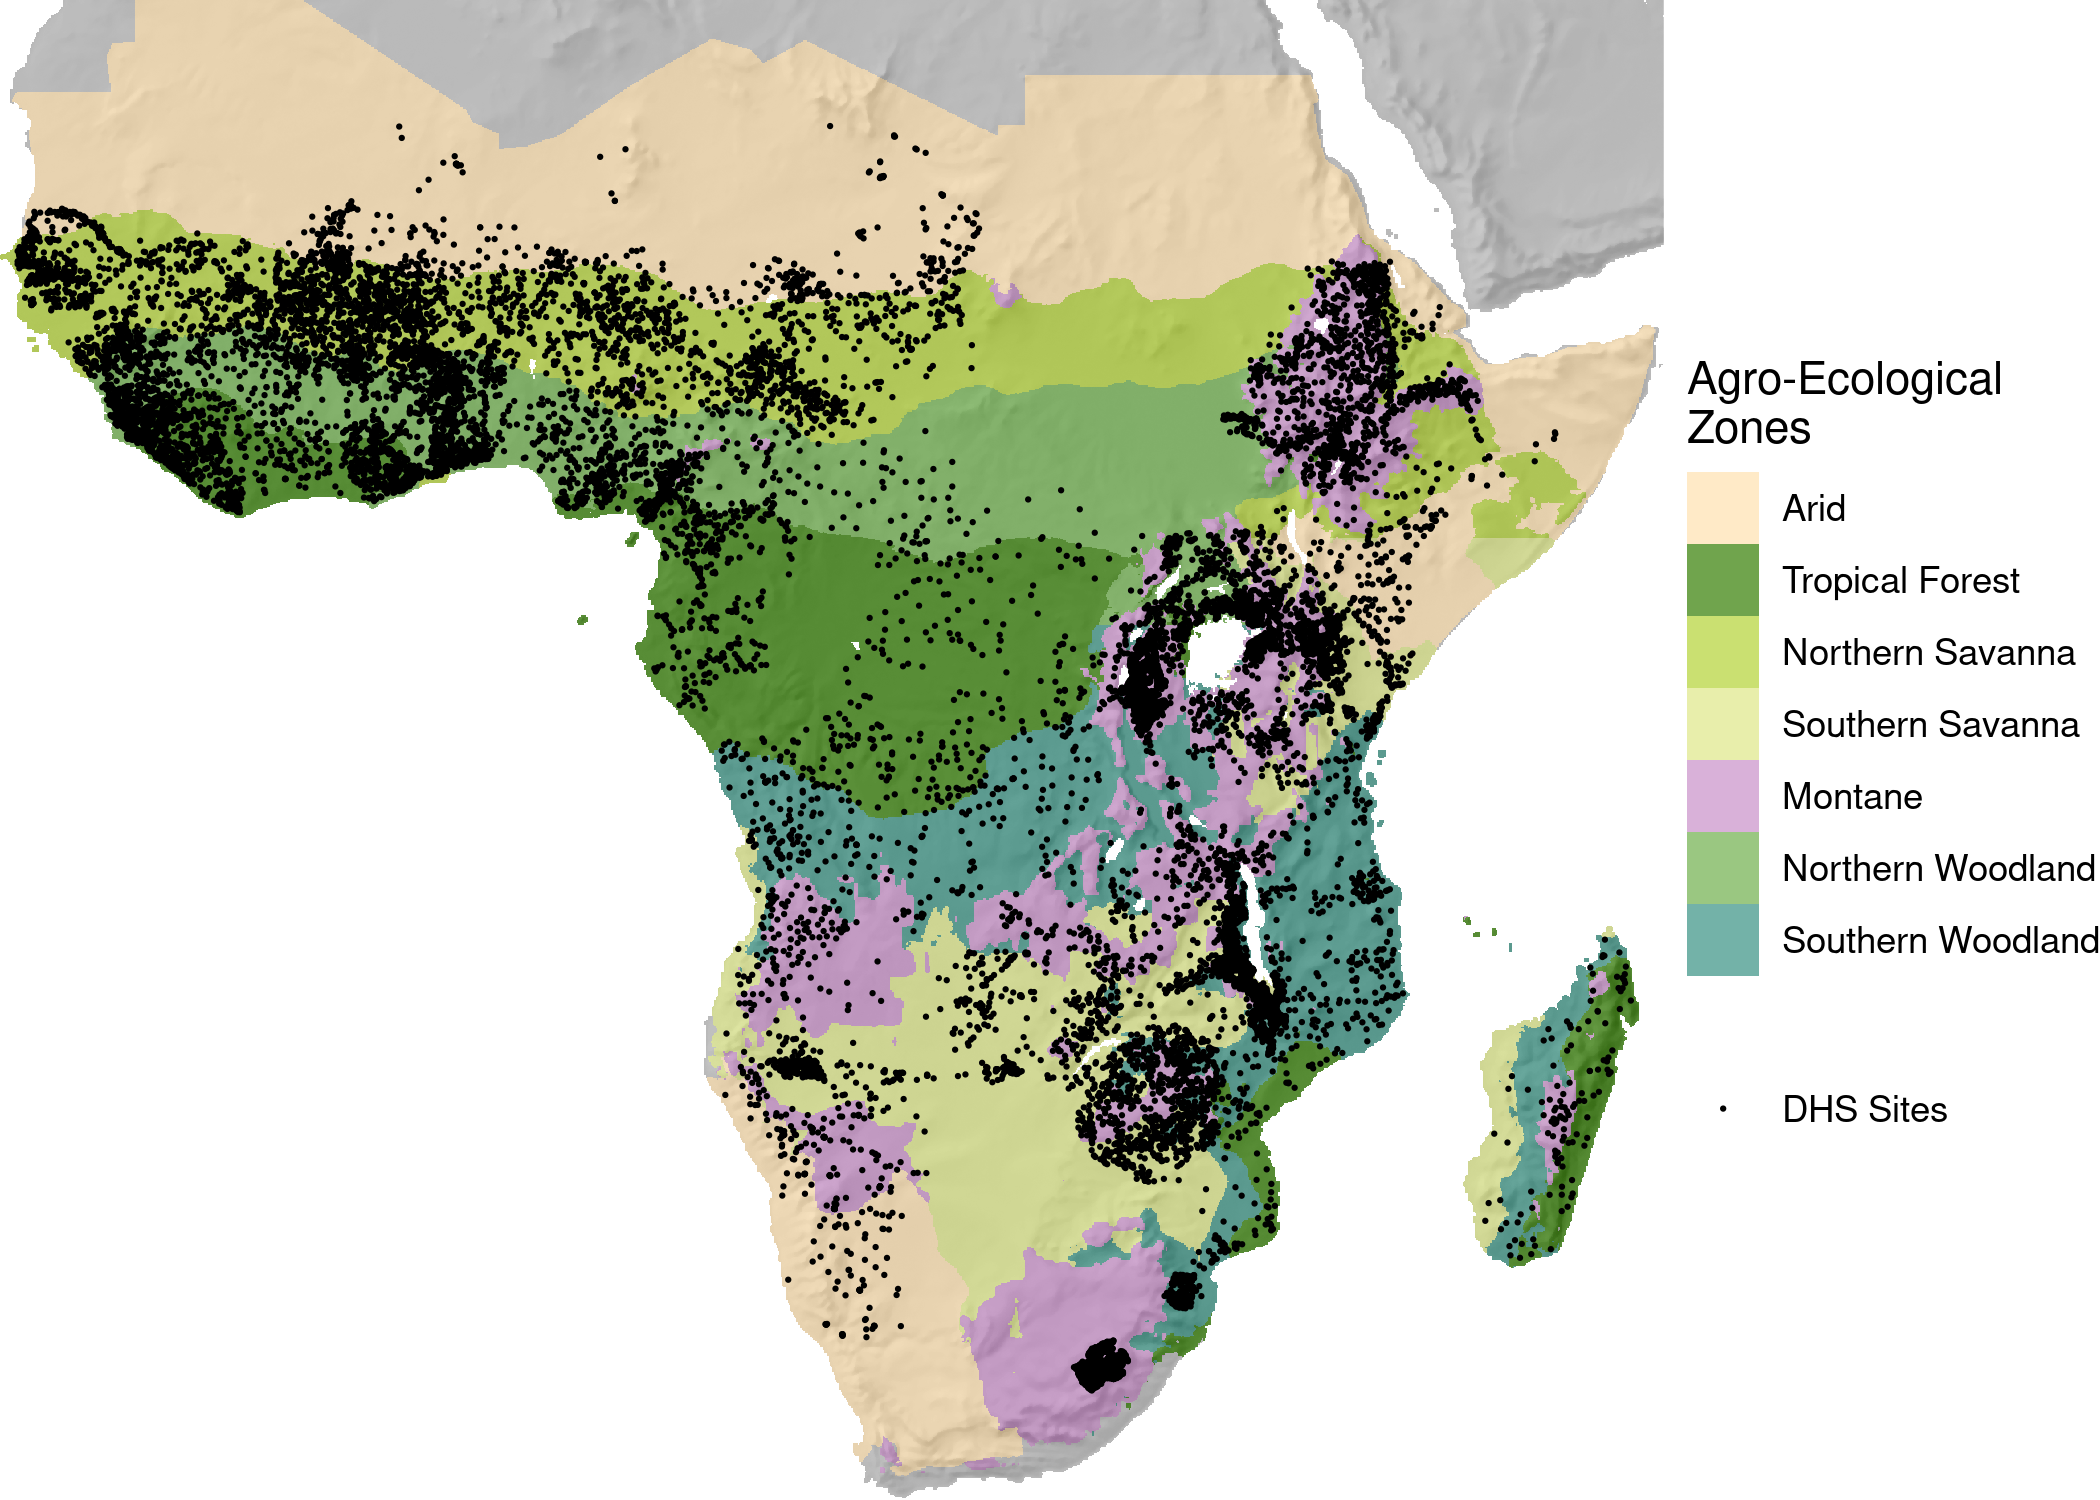
\includegraphics[width=0.8\linewidth]{AEZ_Sites.png}
	\caption{Agro-ecological zones and DHS sites included in the study.}
	\label{fig:AEZmap}
\end{figure}

\section{Methods}
For this analysis we model how access to ecosystem services affects the vulnerability of nutrition to drought in each agro-ecological zone.  We use a special class of Generalized Additive Model (GAM) known as a Varying-Coefficient model \cite{Wood2017} with a nonlinear smooth to model how the impact of droughts on HAZ scores varies according the amount of nearby natural land cover.  Furthermore, we use Covariate Balancing Generalized Propensity Scoring (CBGPS) \cite{imai2014covariate} to control for the effects of other geographic factors that affect drought vulnerability and may be correlated with land cover and land use, including population density, subnational GDP per capita, access to larger cities, international trade.

\subsection{Covariate Balancing Generalized Propensity Scoring}
A number of factors are associated with the presence or absence of uncultivated land cover that also affect drought vulnerability.  Thus, to be able to infer that it is uncultivated areas and the ecosystem services they provide that are having a causal effect on reducing drought vulnerability, it is important to control for these variables.  Propensity score weighting is a popular method to deal with this issue; however, most traditional methods involve a binary treatment variable, which must be dichotomized if it is initially measured in continuous terms \cite{Hirano2003, Robins2000}.  Because our treatment variable, uncultivated land, is continuous, and we have no theoretical priors on how it could be dichotomized, we opt instead to use Covariate Balancing Generalized Propensity Scoring (CBGPS), which can be used for continuous treatments and is more robust to mis-specification \cite{Fong2018}.  Moreover, we use the non-parametric method to estimate the generalized propensity score, which finds weights that leave each confounding variable uncorrelated with the treatment variable, while maximizing the empirical likelihood of observing the data.  The non-parametric approach makes it possible to avoid assumptions about the functional form of the propensity score, but is more computationally costly \cite{Fong2018}.

We balance for demographic and economic factors that can influence both drought vulnerability as well as land cover.  These are: population, from the WorldPop project \cite{Tatem2017}, which can affect land cover by increasing pressure for agricultural production \cite{ouedraogo2010land}, as well as drought vulnerability by increasing access to off-farm labor opportunities but also increasing pressure for resources; subnational GDP per capita \cite{Kummu2018}, which can drive agricultural expansion and deforestation, especially in developing countries \cite{culas2012redd}, while also decreasing drought vulnerability \cite{Carrao2016}; national imports per capita \cite{WorldBank2017}, which can drive agricultural expansion \cite{Meyfroidt2013} while also increasing food access when local food production is low \cite{janssens2020global}; and time to travel distance to major cities \cite{Weiss2018, Uchida2008}, which is an indicator of roads and markets, which can both foster deforestation and agricultural expansion \cite{barber2014roads} as well as buffer child nutrition from the effects of droughts \cite{Shively2017}.

After using the non-parametric CBGPS methodology to generate weights for each of these variables with respect to the availability of uncultivated land, we tested to see whether the correlation between these variables and uncultivated land cover decreased \cite{Fong2018}.  We run the algorithm separately for each AEZ in our analysis.  To conduct the balancing we use the CBPS package for R \cite{Fong2018a}, with the default value of $0.1/N$ for the tuning parameter $\rho$, which moderates the trade-off between completely reducing correlation and avoiding extreme outlier weights.  Finally, as a robustness check, we assessed whether censoring extreme weights at the 80th and 90th percentile would affect our model estimates.

\subsection{Modeling Framework}
Having derived weights for the propensity of each observation to have uncultivated land in its vicinity, we then model nutrition outcomes as a function of the local 24-month SPEI score, where the coefficient for SPEI is modeled as a function of uncultivated land cover, controlling for typical household and individual factors as well as the spatially-varying baseline rate of malnutrition using a spherical spline.  This is a specific form of Generalized Additive Model \cite{Hastie1986} known as a varying coefficient model \cite{Wood2017}.  Specifically, or model takes the following form:

\begin{equation}
  y_{ija} = \beta_0 + \beta X_{ija} + s(lat_{ja}, lon_{ja}) + f_{a}(\nu_{ja}) spei_{ja} + \epsilon_{ija} \label{eqn:GAM}
\end{equation}

Where $i$ indexes individuals, $j$ indexes DHS sites, and $a$ indexes agro-ecological zones. In this model, $y_{ija}$ is a given child's HAZ score, $\beta_0$ is a fixed intercept, $X_{ija}$ is a matrix of individual and household covariates, modified by a vector of coefficients $\beta$, $s(lat_{ja}, lon_{ja})$ is a spatially varying effect estimated by a spherical spline basis \cite{Wahba1982}, and $f_{a}()$ is a spline function that determines coefficient for the 24-month SPEI based on the amount of uncultivated land cover $\nu_{ja}$, estimated separately for each AEZ.  The basis we use for the varying coefficient function $f()_{a}$ is estimated using thin plate splines \cite{Duchon1977}, and the smoothing parameter for this smooth is estimated through Generalized Cross Validation (GCV) \cite{Wood2017}.

To more precisely estimate the effect of drought on child stunting, we control for a number of individual and household factors that affect stunting outcomes.  These are: the child's age, the child's birth order, the size of the household the child lives in, the sex of the child, the mother's years of education, the household's toilet facility, the interview year, the age of the household head, the sex of the household head, the month of the child's birth, which can be a source of measurement error in estimating the child's HAZ score \cite{larsen2019misreporting}, as well as the household wealth index, normalized to be comparable across surveys \cite{Rutstein2014c}.

\subsection{Estimating the Contribution of Uncultivated Land to Drought-Resilient Nutrition and Comparison with Other Conservation Priorities}
To estimate the contribution of uncultivated land to nutrition outcomes, we use our regression results to estimate two scenarios in areas where natural land cover was found to buffer children from the effects of drought: one estimating the impact of drought on child HAZ scores based on current levels of natural land cover, and one counter-factual scenario estimating the impact of drought on child HAZ scores if natural land cover if there were no nearby natural land cover.  The difference between the predicted HAZ scores from the baseline scenario versus those from a no-natural-land-cover scenario provides an estimate of where and how much local nutrition is supported by local ecosystem services.

While our model estimates the change in mean HAZ scores under drought conditions, the increase in rates of stunting is a more familiar metric for policymakers.  Thus, we convert our model estimates of changes in mean HAZ score to changes in rates of stunting. Given that HAZ scores are normally distributed and the rate of stunting is the percentage of children under 5 years old with an HAZ score of less than -2, it is possible to covert changes in mean HAZ scores into increases in rates stunting given prevailing mean HAZ scores, which can in turn be derived from prevailing rates of stunting and the standard deviation of HAZ scores.  Thus, for estimates of current HAZ scores, we use data from a recent analysis of rates of stunting in Africa \cite{Osgood-Zimmerman2018}.  Because this analysis estimated rates of stunting for the years 2000-2015, we the annualized rate of change (AROC) trend extrapolation method common in epidemiology to conduct a pixel-wise forecast to the year 2020 \cite{Fullman2017, Osgood-Zimmerman2018}.  For standard deviation, overall standard deviations in HAZ scores have been observed to vary independently of mean HAZ scores \cite{Mei2007} and to not change significantly over time.  Therefore, we simply use the standard deviation for our dataset (1.62), which matches previous literature on the standard deviation of HAZ scores in surveys in Africa \cite{Mei2007}.  Having determined the changes in rates of stunting between a baseline scenario and a scenario without uncultivated land cover, we then use gridded age-specific population data \cite{Tatem2017} to determine the number of children additional children in a given location that would be stunted during a drought with and SPEI score of $-2$ in the absence of uncultivated land.

Finally, in order to highlight areas where environmental conservation can achieve multiple climate-relevant conservation goals, we compare our predictions of where conservation interventions can contribution to climate-resilient nutrition with a map of conservation priorities to preserve biodiversity under climate change \cite{hannah2020}.  This comparison map of biodiversity priorities was the result of modeling the expected habitat ranges of vertebrate and plant species in the period 2060-2080 under the Representative Concentration Pathway (RCP) 8.5 \cite{hannah2020}.

\section{Results}
\subsection{Covariate Balancing}
After estimating weights using CBGPS, the correlation between uncultivated land cover and the various confounding variables that we attempted to control for was significantly reduced.  Table \ref{tab:CBPSsum} shows the reduction in correlation between these variables based on the weighting.

\begin{table}[h!]
	\begin{center}
		\begin{tabular}{r | c c c c c c c c c c c c c c c c }
&	\multicolumn{2}{c}{Import Value} &	\multicolumn{2}{c}{Population} &	\multicolumn{2}{c}{Subnational}	&	\multicolumn{2}{c}{Time to Travel}	\\
&	\multicolumn{2}{c}{Per Capita} &	\multicolumn{2}{c}{Density} &	\multicolumn{2}{c}{GDP Per Capita}	&	\multicolumn{2}{c}{to Major City}	\\
	\cmidrule(lr){2-3}\cmidrule(lr){4-5} \cmidrule(lr){6-7}\cmidrule(lr){8-9}
      AEZ	&	\textit{Unwgtd.}	&	\textit{Wgtd.}	&	\textit{Unwgtd.}	&	\textit{Wgtd.}	&	\textit{Unwgtd.}	&	\textit{Wgtd.}	&	\textit{Unwgtd.}	&	\textit{Wgtd.}	\\
\hline									
Arid	&	0.22	&	0.01	&	0.27	&	0 &	0.16	&	-0.01	&	-0.15	&	0	\\
Tropical Forest	&	0.1	&	0.1	&	-0.47	&	0.04&	0.19	&	0.08	&	0.31	&	-0.03	\\
Montane	&	0.37	&	0.03	&	-0.64	&	-0.14&	0.17	&	-0.04	&	0.33	&	0.12	\\
Northern Savanna	&	0.02	&	0.03	&	-0.45	&	0.02&	-0.16	&	0.02	&	0.24	&	0.01	\\
Northern Woodland	&	0.16	&	-0.03	&	-0.41	&	-0.01&	-0.03	&	-0.04	&	0.12	&	0.03	\\
Southern Savanna	&	0.45	&	0.01	&	-0.62	&	-0.03&	0.47	&	0.02	&	0.24	&	0.05	\\
Southern Woodland	&	0.46	&	-0.09	&	-0.7	&	0.18&	0.22	&	0.06	&	0.17	&	0.05	\\	
		\end{tabular}
    \caption{Summary of correlation between uncultivated land cover and confounding variables with no weighting (\textit{Unwgtd.}) and after weighting using CBGPS (\textit{Wgtd.}).}
	\label{tab:CBPSsum}
	\end{center}
\end{table}

\subsection{Role of Natural Land Cover in Moderating Drought by AEZ}

Having estimated the model, our main parameters of interest are the varying coefficients for how uncultivated land cover affects the impact of drought in each AEZ.  Thus, we graph those effects here in Figure \ref{fig:naturaleffect}, and include full model results in the Appendix.

\begin{figure}[h!]
	\begin{center}
	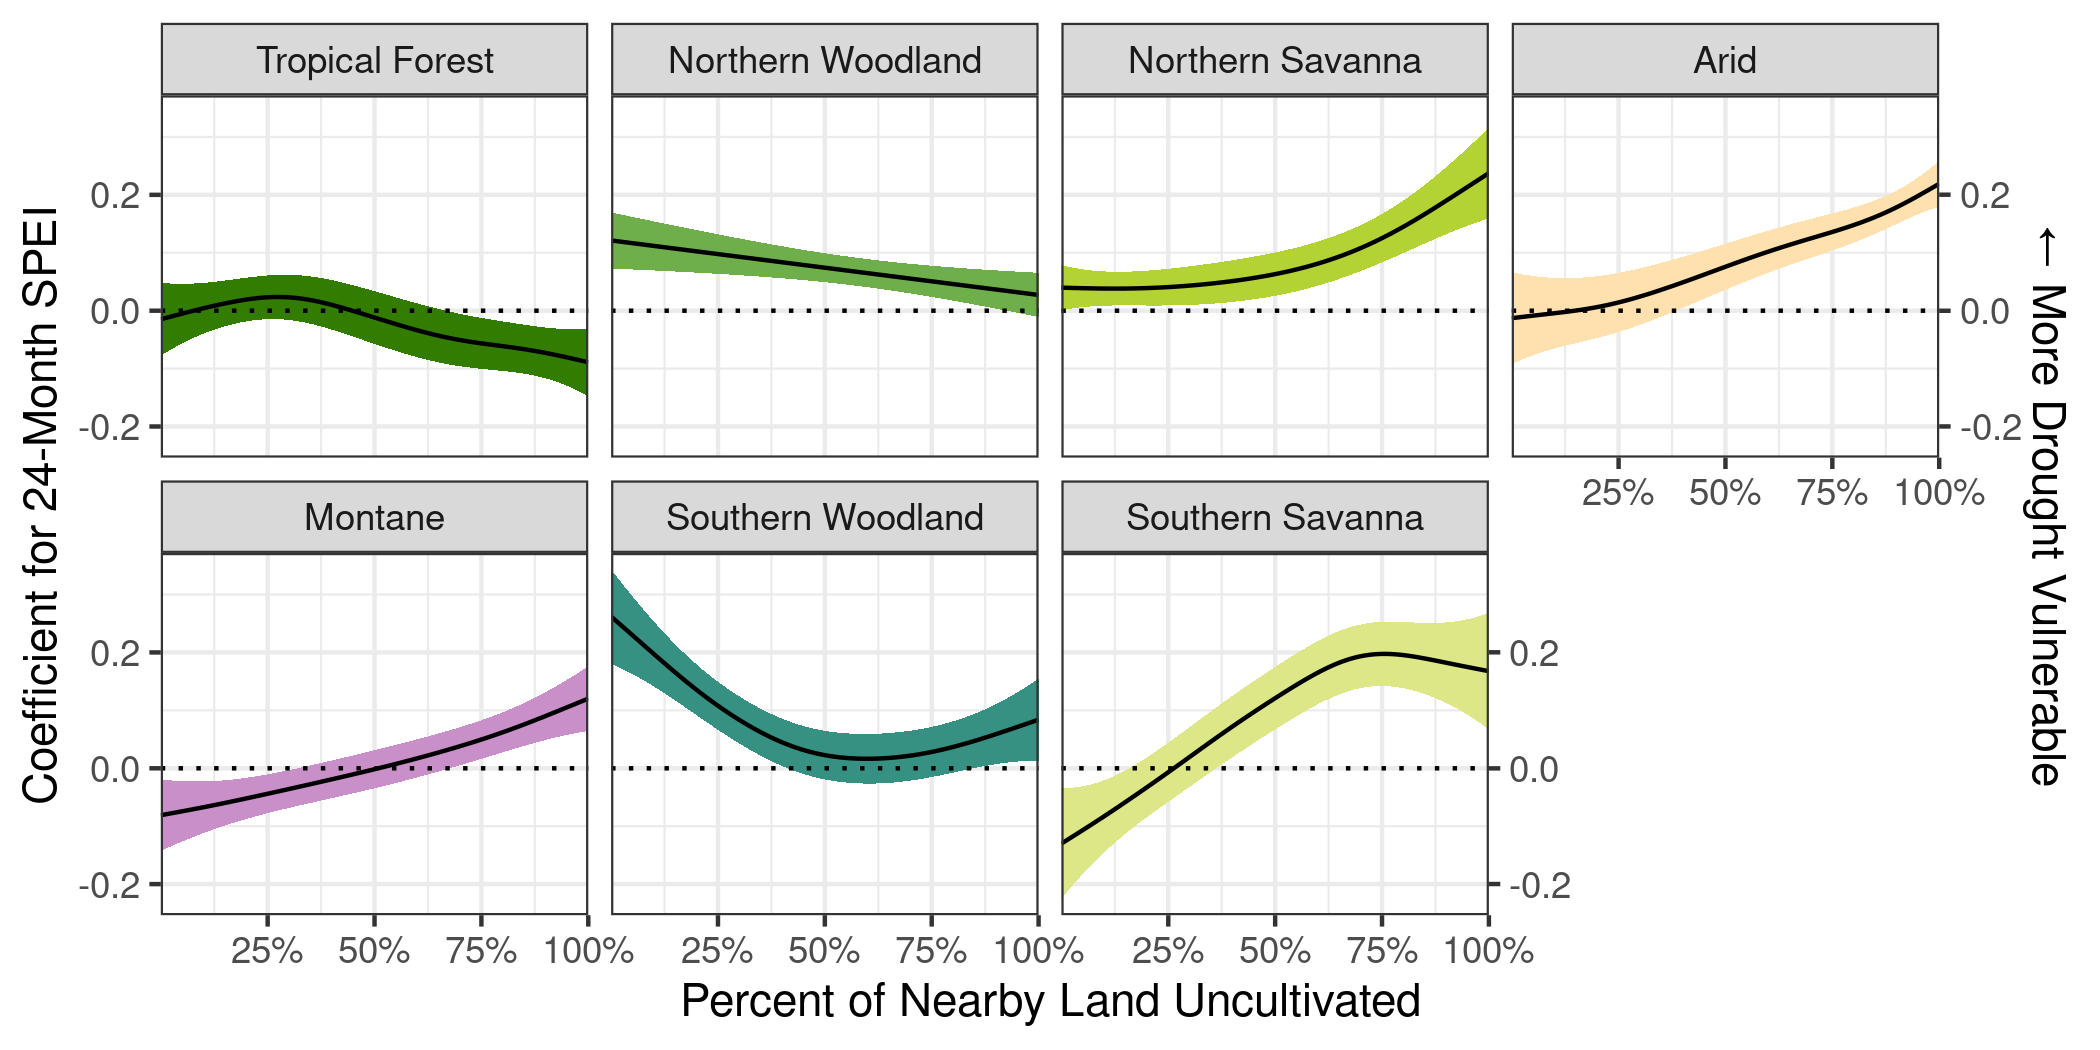
\includegraphics[width=\linewidth]{AEZ_effects.png}
	\end{center}
	\caption{Effect of droughts on child nutrition outcomes by agro-ecological zone (AEZ), varying as a function of the percent of nearby land cover that is uncultivated.  In arid, savanna, and montane zones, more natural land cover is associated with greater drought vulnerability, while in woodland zones, more natural land cover is associated with less drought vulnerability.  Error bands indicate the 95\% confidence interval.}
	\label{fig:naturaleffect}
\end{figure}

Figure \ref{fig:naturaleffect} shows how the coefficient for the 24-month SPEI varies as a function of the percent of nearby natural land cover.  The error band around the parameter indicates the 95\% confidence interval.  Thus, areas where the error band does not cross 0 (at the dotted line) indicates that, at that level of uncultivated land cover, precipitation anomalies have a statistically significant effect on child nutrition outcomes.

In many AEZs, the coefficients slope upwards, indicating that increasing rates of natural land cover are associated with a larger coefficient and thus greater drought vulnerability.  However, in the woodland AEZs of both northern and southern Africa, increasing rates of natural land cover are associated with a smaller coefficient and thus less drought vulnerability.  At low levels of natural land cover in both northern and southern sub-forest Africa, a moderate drought (SPEI = -2) decreases mean HAZ scores by 0.2 to 0.4, whereas at high levels of natural land cover, a similar drought has no significant effect on nutrition outcomes.

\subsection{Modeling Ecosystem Service Dependence Over Space}
Our model indicates that in semi-humid woodland parts of Africa, uncultivated land buffers child nutrition from the effects of drought.  Thus, focusing on these AEZs, we contextualize the model by estimating the increase in the number of under-5 children that would become stunted in the absence of natural land cover during a drought.

\begin{figure}[h!]
	\begin{center}
		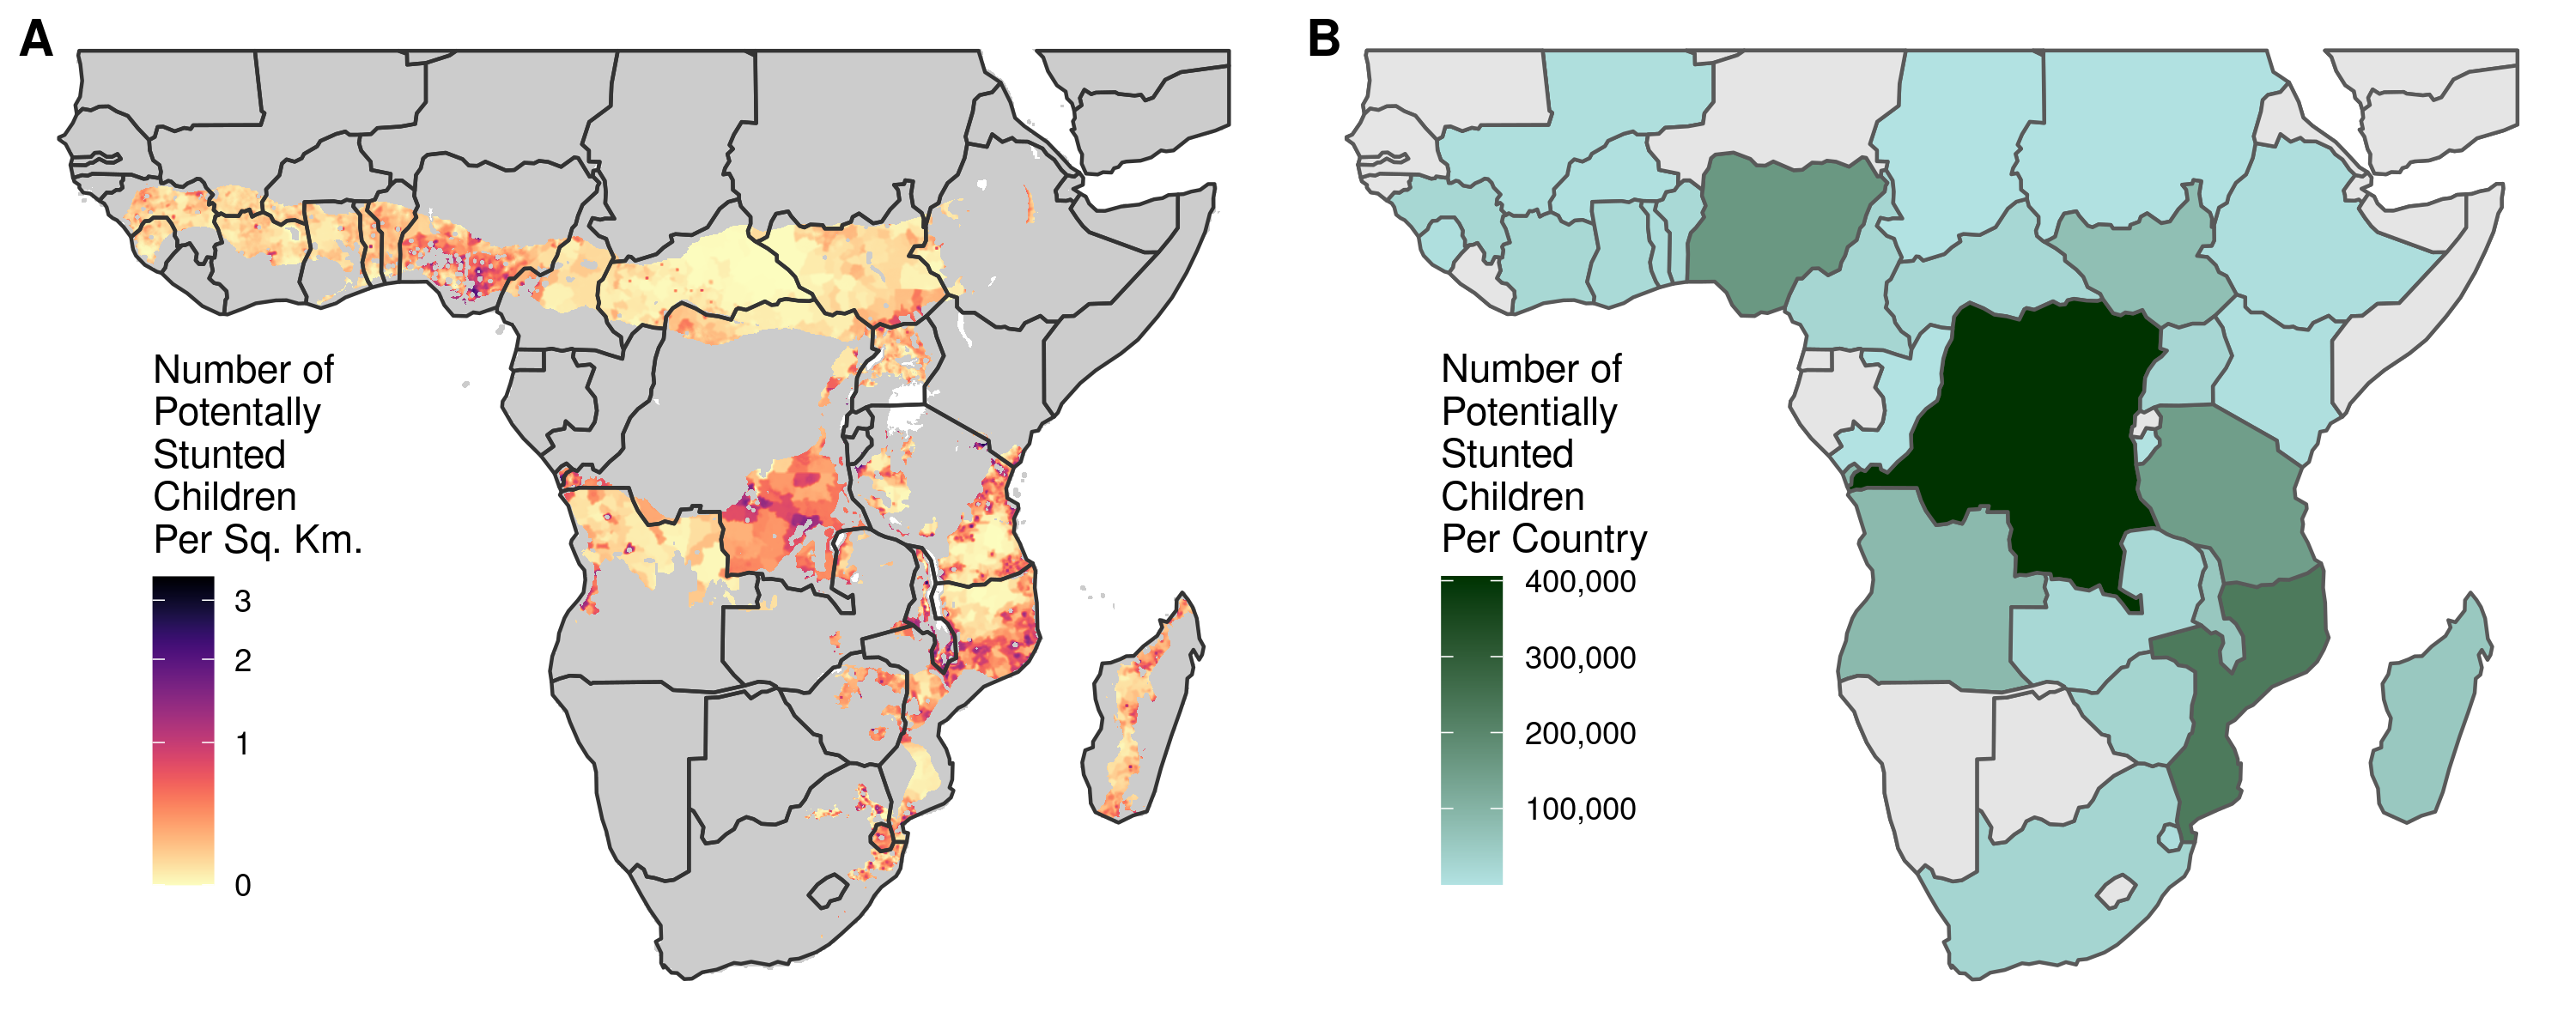
\includegraphics[width=\linewidth]{AfricaEffect.png}
    \caption{\textbf{A}) The number of additional children per square kilometer who would become stunted during a drought in the absence of natural land cover.  \textbf{B}) The same figure, aggregated by country rather than calculated per square kilometer.}
		\label{fig:AfricaEffect}
	\end{center}
\end{figure}

Figure \ref{fig:AfricaEffect} shows the number of additional children that would become stunted during a drought in the absence of natural land cover, based on current land cover conditions and rates of stunting, estimated per square kilometer and aggregated to the country level.  The areas that would see an increase in stunting in the absence of local natural land cover were mostly the woodlands of Africa, such as the Guinean forest-savanna mosaic of Northern and Western Africa as well as the Miombo woodlands of Southern Africa. Examining the potential increase in stunted child under drought in each of these AEZs shows that many of them would be located in the woodlands of southern DRC, central Nigeria as well as in parts of Mozambique, Malawi, and southern Tanzania.  Throughout Africa, an additional 1.5 million children would be stunted under drought without local ecosystem services.  The countries that currently see the most benefit to child nutrition from local ecosystem services are the DRC, Mozambique, Nigeria, and Tanzania.

\subsection{Comparison With Biodiversity Conservation Priorities}

\begin{figure}[h!]
	\begin{center}
		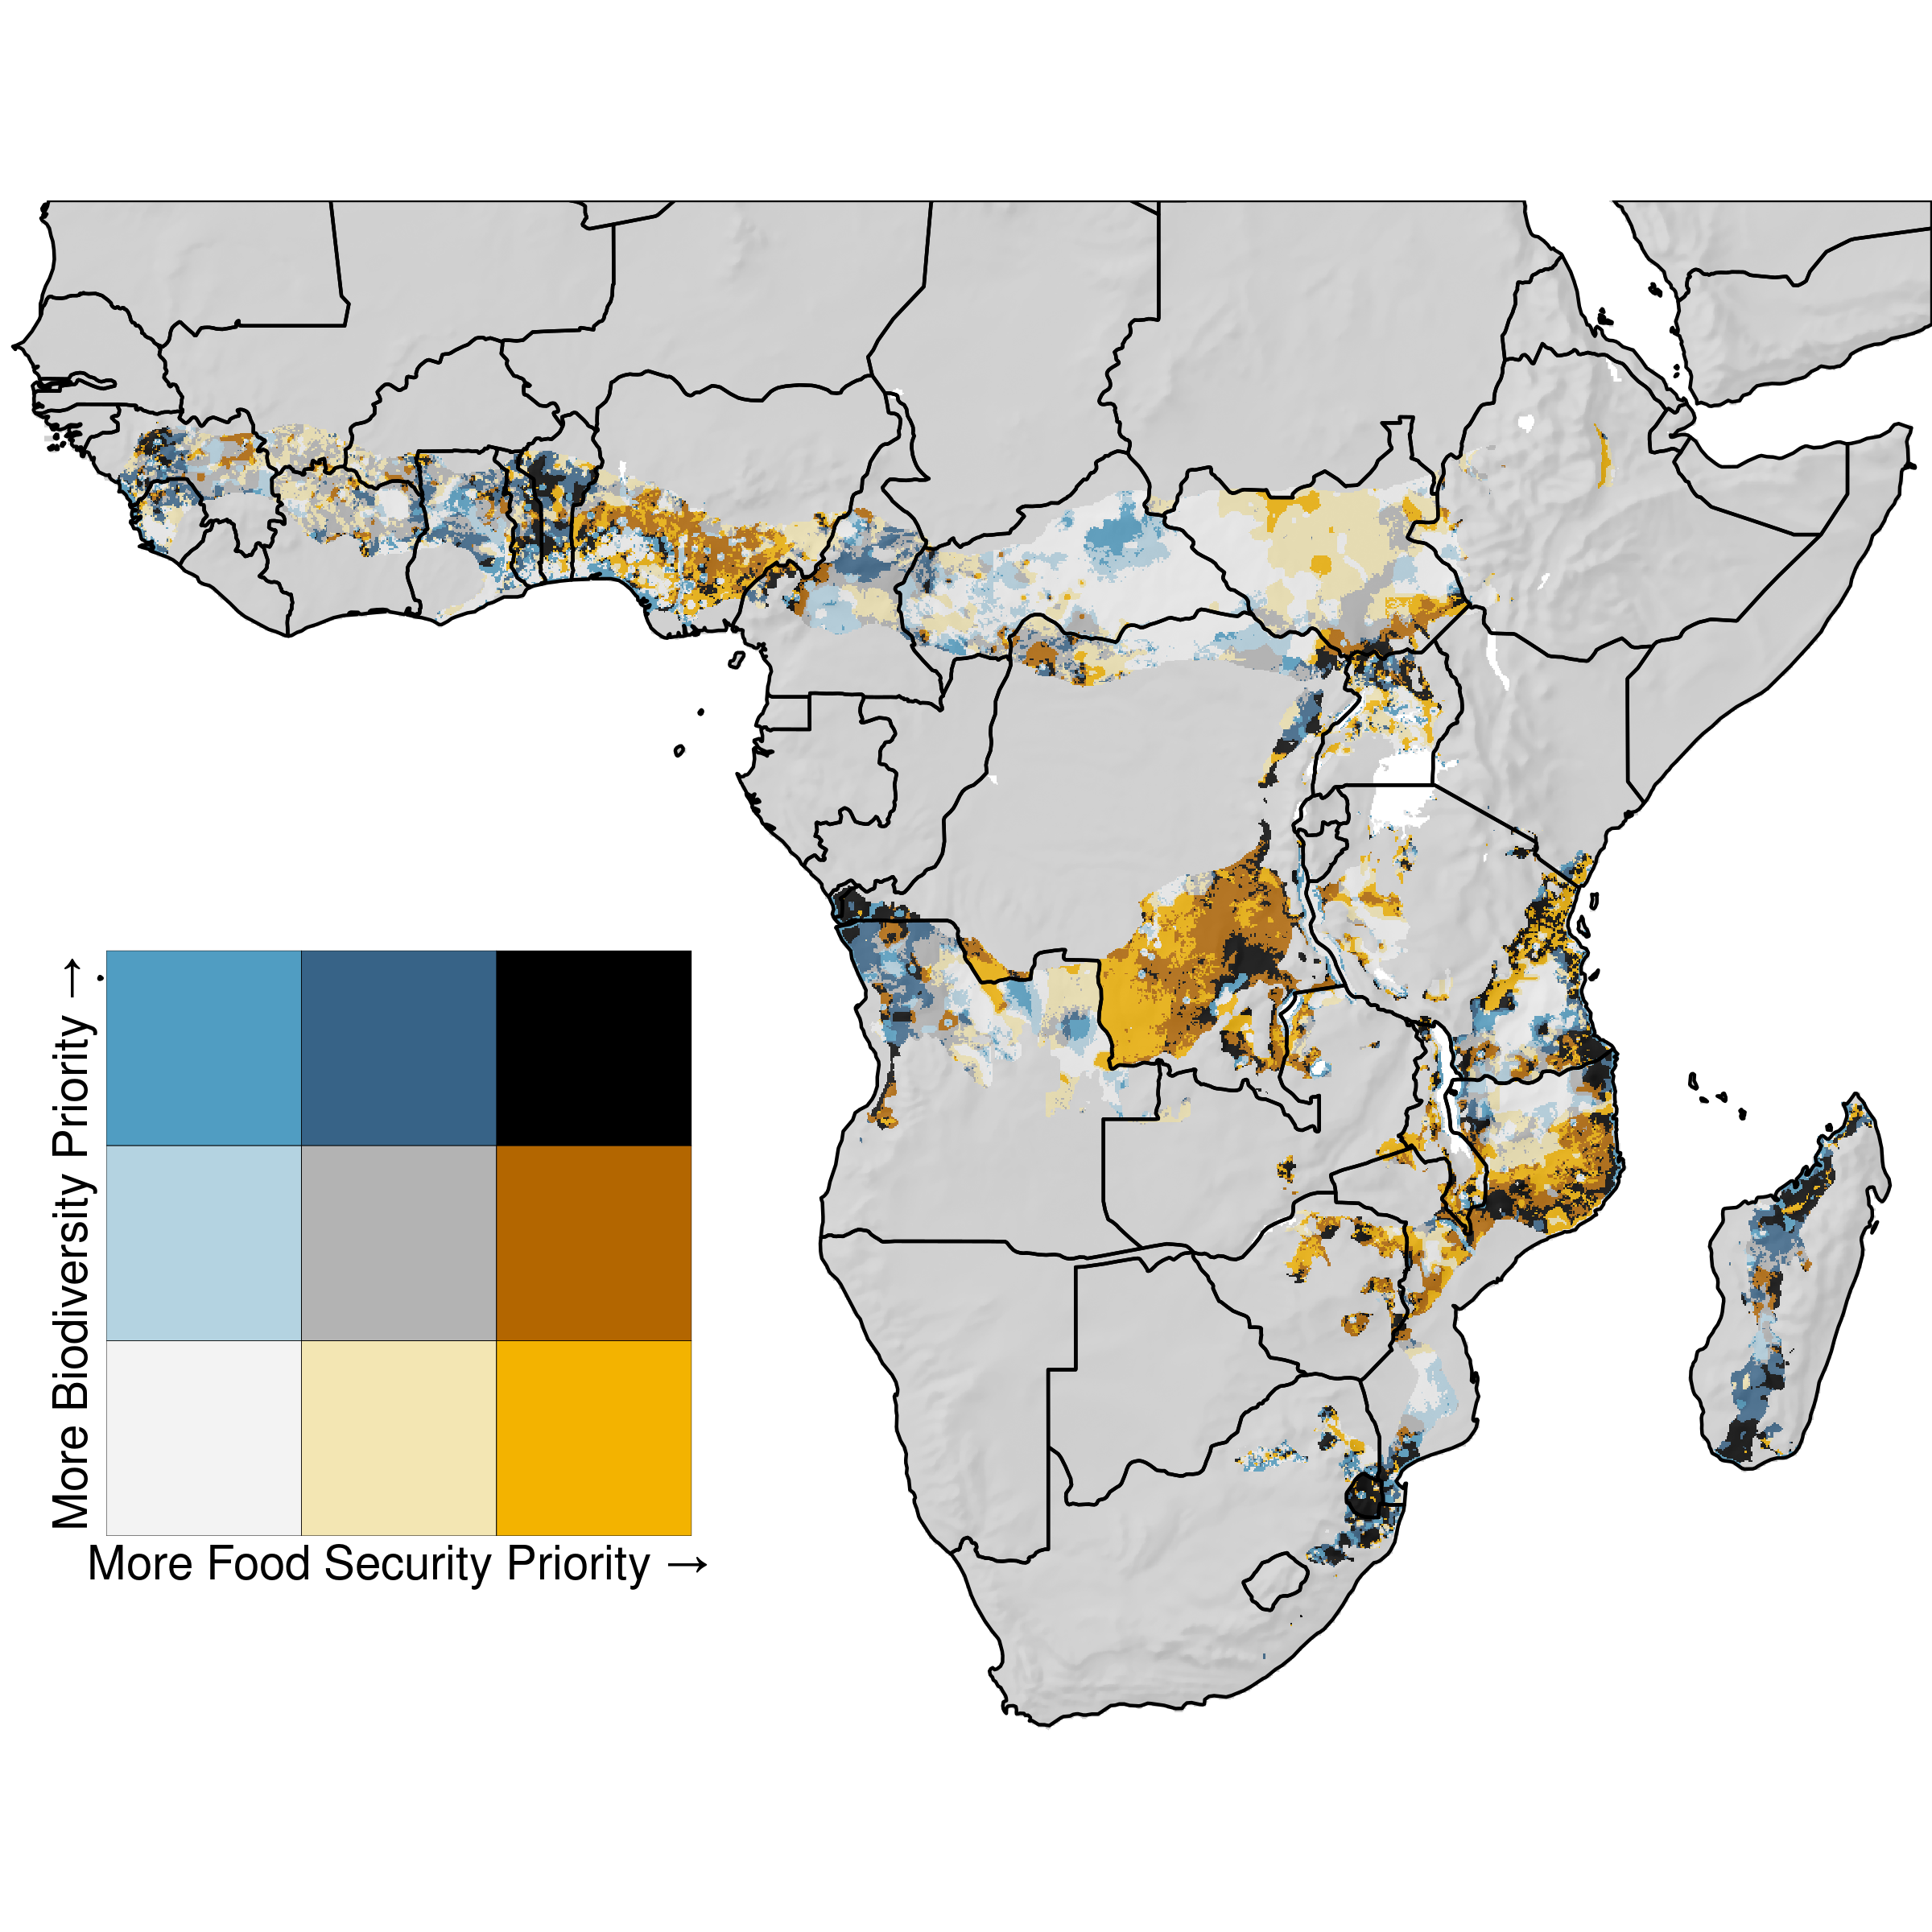
\includegraphics[width=0.8\linewidth]{Bivariate_Map.png}
		\caption{Map of the intersection of areas that are a priority for conservation under climate change for two goals of preserving biodiversity and ensuring resilient food security.  Areas in blue are important for biodiversity but not food security, areas in orange are important for food security but not biodiversity, and areas in black are important for both food security and biodiversity.}
		\label{fig:Bivariate_Map}
	\end{center}
\end{figure}

Examining the overlap between two conservation goals under climate change highlights landscapes throughout Africa where conservation interventions could meet both biodiversity and food security goals (See Figure \ref{fig:Bivariate_Map}).  These included areas in Benin, northern Uganda and southern South Sudan, the Katanga region of the DRC, the mouth of the Congo River, the coastal area the Mozambique-Tanzania border, Eswatini and nearby parts of Mozambique and South Africa, as well as parts of Madagascar. There are also many landscapes throughout the continent where conservation could work towards one of the two goals without fully supporting the other.

\section{Discussion}

This paper assessed how the prevalence of uncultivated land cover moderates the impact of drought on child nutrition outcomes throughout several agro-ecological zones in Africa.  We took care to control for the potential confounding effects of several factors that could influence both the presence of uncultivated land as well as drought vulnerability.  We found that the manner in which natural land cover moderated the effect of drought on child nutrition outcomes varied by AEZ, and that there is an observable safety net effect in semi-humid woodland landscapes throughout the continent, although natural land cover is associated with greater drought vulnerability in arid and savanna AEZs.  Finally, examining a counter-factual scenario of the impact of droughts without uncultivated land cover and the ecosystem services it provides shows that millions of children are dependent on ecosystem services to meet their nutrition needs in times of drought.

A major contribution of this paper to the literature is its scale.  Most other studies of the role in ecosystem services in buffering human well-being from climate shocks tends to focus on case studies \cite{Debela2012} as well as use hypothetical scenarios \cite{Robledo2012} or retrospective analyses \cite{Muller2008}.  This paper provides a large scale analysis of observed nutrition outcomes during varying levels of drought as well as across sites with varying access to ecosystem services.  Performing an analysis at this scale allowed us to compare how uncultivated land affects drought vulnerability across many agro-ecological zones and aid in conservation priority setting across Africa.

One of the only other multinational analyses of the role of ecosystem services as a buffer during shocks found that households did not rank forest resources as a very important resource during shocks \cite{Wunder2014}.  While Wunder et al.'s results seem to contradict our results, their analysis differed in significant ways from ours: they focused on forests rather than all uncultivated land cover types, they focused on a variety of types of shocks beyond just drought, and they asked households retrospectively about previous shocks rather than observing them \textit{in situ}.  Thus, there are several reasons why we observed natural land cover as playing as significant effect in buffering households from drought in woodland landscapes while Wunder et al. did not find such an effect.  For example, it may be that households do not pivot towards forest resourced during drought; rather, households that are always using forest resources are simply less affected by agricultural shocks like drought. Additionally, by focusing only on forest resources like timber, Wunder et al. were unable to explore the benefit that supporting and regulating ecosystem services have on local agricultural production.  

An important aspect of this analysis was using weighting to ameliorate the effects of potential confounding variables.  Because we controlled for the effects of several demographic and economic variables, we can more confidently ascribe the observed drought mitigation to the land cover itself rather than to another factor that is correlated with land cover.  However, given that weighting each covariate to achieve a correlation of perfectly 0 would be either impossible or would require extreme weights, we did not reduce the correlation between our confounding variables and natural land cover all the way to 0 (See Table \ref{tab:CBPSsum}).  Nevertheless, we diminished the correlation to the extent that a causal interpretation of the observed mitigation effect of natural land cover is now more plausible. Moreover, we validated the robustness of our weighting by censoring the weights at the 80th and 90th percentile and getting similar results, confirming that the observed effects were not due to extreme weights on a small number of observations.

While the model estimated the moderating effect of natural land cover on drought vulnerability as varying across AEZs, we found that uncultivated land cover played a similar function in ecologically similar zones.  In both northern-hemisphere and southern-hemisphere savanna zones, greater uncultivated land cover was associated with greater drought vulnerability.  On the other hand, in the ecologically similar but geographically disjoint woodland zones, natural land cover had a safety net effect during drought.  The fact that ecologically similar AEZs were modeled as having similar effects in terms of drought vulnerability, even though they were modeled with independently estimated smoothing splines, suggests that this effect is real and is ecologically based.

These findings suggest that uncultivated land does not act as a safety net for livelihoods in arid and savanna environments during droughts, and that in these areas, more uncultivated land is in fact associated with more drought vulnerability.  This could be due to the fact that much of the vegetation in these areas is annual grasses, which, like annual crops, are highly affected by droughts because they are less shaded and do not have deep taproots like woody vegetation in more humid areas.  Moreover, arid and savanna landscapes provide less wild foods or other provisioning services compared to other vegetation regimes, and so are primarily used for grazing livestock.  Similarly, many regulating and supporting ecosystem services provided by natural land cover, such as wind breaking, shading and temperature regulation, and moisture retention are specifically a function of trees \cite{Reed2016}.  Thus, areas lacking in trees may not be able to provide the safety net effect that more forested areas have.  For very humid and mesic areas with closed-canopy tropical forests, other the other hand, drought does not have a significant effect on stunting at level of uncultivated land cover.  Our results suggest that, in this AEZ, nutrition is unaffected even if precipitation is well below historic norms and, if anything, increased stunting may be caused by excess rainfall in certain landscapes.  Overall, our results indicate that the open-canopy woodlands of Africa present a middle ground, where rainfall levels are low enough that a drought can affect food production and lead to increases in stunting, but rainfall is still high enough that in uncultivated areas there is both the biodiversity and biomass to provide a safety net.  Moreover, these mixed woodland landscapes between open grasslands and dense forests can support a wide variety of natural land cover types, and farmers frequently shape the landscape to maximize a diversity of food sources \cite{fairhead1996misreading}.

While the association between natural land cover and reduced drought vulnerability in certain AEZs is certainly suggestive that people are relying on ecosystem services as a safety net, this analysis cannot speak to the particular pathways through which people are benefiting from nature.  For example, the relative importance of provisioning ecosystem services such as wild foods versus regulating services such as shading to prevent moisture loss cannot be ascertained.  Nevertheless, previous work in Africa has found that greater natural land cover is associated with greater collection of wild foods and nonfood Non-Timber Forest Products, suggesting that provisioning ecosystem services are a part of the pathway \cite{Cooper2018a}.

Finally, we used our model to map where conservation interventions could have the largest impact on reducing child malnutrition under an increasingly drought-prone climate, and compared this map with the results of a recent study examining conservation priorities for conserving plant and vertebrate diversity under climate change \cite{hannah2020}.  The resulting map (See Figure \ref{fig:Bivariate_Map}) highlights many landscapes where conservation could synergistically help meet SDGs 2 and 15 - to improve food security and preserve biodiversity.  Aside from being in woodland AEZs, these landscapes tend to be mildly populated areas, often near uninhabited existing national parks and protected areas, such as Pendjari National Park in Benin, Murchison Falls National Park in Uganda, or Kruger National Park and Parque Nacional de Limpopo in Mozambique and South Africa.  In these areas, people-centered conservation schemes such as community based forest management could support better nutrition and biodiversity outcomes under a changing climate \cite{bray2003mexico}.

\section{Conclusion}
These findings are have important implications for the study of food security, climate change vulnerability, and environmental conservation.  We showed that nature can be a critical part of reducing climate change vulnerability, but the specific role that nature plays is highly context-specific.  While mapping ecosystem services has traditionally focused on variables like carbon stocks and biodiversity hotspots, this analysis shows that the contributions of nature to food security can also be mapped to support improved nutrition.  Given the increasing threat of a more drought prone world under climate change \cite{Dai2013} combined with the severe precarity of Africa's agrarian poor, dampening the effects of drought and providing alternative food and income sources when agriculture fails may indeed be one of nature's most important contributions to people.

\bibliographystyle{apalike}
\bibliography{library}

\setcounter{section}{0}
\renewcommand{\thetable}{A\arabic{section}}
\section*{Appendix} \label{AppendixA}
\setcounter{table}{0}
\setcounter{figure}{0}
\renewcommand{\thetable}{A\arabic{table}}
\renewcommand{\thefigure}{A\arabic{figure}}

\section{Full Model Results}

\begin{longtable}{l c }
\hline
 &  \\
\hline
\endfirsthead
\hline
 &  \\
\hline
\endhead
\hline
\endfoot
\hline
\multicolumn{2}{l}{\scriptsize{$^{***}p<0.001$, $^{**}p<0.01$, $^*p<0.05$}}\\
\caption{Statistical models}
\label{table:coefficients}
\endlastfoot
age                              & $-0.02^{***}$  \\
                                 & $(0.00)$       \\
birth\_order                     & $0.01^{***}$   \\
                                 & $(0.00)$       \\
hhsize                           & $-0.00$        \\
                                 & $(0.00)$       \\
sexFemale                        & $-17.07^{***}$ \\
                                 & $(1.44)$       \\
sexMale                          & $-17.19^{***}$ \\
                                 & $(1.44)$       \\
mother\_years\_ed                & $0.03^{***}$   \\
                                 & $(0.00)$       \\
toiletNo Facility                & $-0.16^{***}$  \\
                                 & $(0.01)$       \\
toiletOther                      & $-0.14^{***}$  \\
                                 & $(0.03)$       \\
toiletPit Latrine                & $-0.13^{***}$  \\
                                 & $(0.01)$       \\
interview\_year                  & $0.01^{***}$   \\
                                 & $(0.00)$       \\
as.factor(calc\_birthmonth)2     & $-0.02$        \\
                                 & $(0.02)$       \\
as.factor(calc\_birthmonth)3     & $0.04^{*}$     \\
                                 & $(0.02)$       \\
as.factor(calc\_birthmonth)4     & $0.03^{*}$     \\
                                 & $(0.02)$       \\
as.factor(calc\_birthmonth)5     & $0.03^{*}$     \\
                                 & $(0.02)$       \\
as.factor(calc\_birthmonth)6     & $0.15^{***}$   \\
                                 & $(0.02)$       \\
as.factor(calc\_birthmonth)7     & $0.11^{***}$   \\
                                 & $(0.02)$       \\
as.factor(calc\_birthmonth)8     & $0.18^{***}$   \\
                                 & $(0.02)$       \\
as.factor(calc\_birthmonth)9     & $0.17^{***}$   \\
                                 & $(0.02)$       \\
as.factor(calc\_birthmonth)10    & $0.23^{***}$   \\
                                 & $(0.02)$       \\
as.factor(calc\_birthmonth)11    & $0.23^{***}$   \\
                                 & $(0.02)$       \\
as.factor(calc\_birthmonth)12    & $0.44^{***}$   \\
                                 & $(0.02)$       \\
head\_age                        & $0.00^{***}$   \\
                                 & $(0.00)$       \\
head\_sexMale                    & $-0.07^{***}$  \\
                                 & $(0.01)$       \\
wealth\_norm                     & $0.54^{***}$   \\
                                 & $(0.02)$       \\
AEZ\_newafr.forest.4             & $-0.11^{***}$  \\
                                 & $(0.03)$       \\
AEZ\_newafr.high.7               & $-0.22^{***}$  \\
                                 & $(0.03)$       \\
AEZ\_newnafr.sav.5               & $0.00$         \\
                                 & $(0.02)$       \\
AEZ\_newnafr.subforest.8         & $0.03$         \\
                                 & $(0.03)$       \\
AEZ\_newsafr.subforest.9         & $0.06^{*}$     \\
                                 & $(0.03)$       \\
AEZ\_newseafr.sav.6              & $-0.17^{***}$  \\
                                 & $(0.03)$       \\
EDF: s(latitude,longitude)       & $45.17^{***}$  \\
                                 & $(49.00)$      \\
EDF: s(natural):afr.arid.123     & $3.24^{***}$   \\
                                 & $(3.74)$       \\
EDF: s(natural):afr.forest.4     & $3.20^{**}$    \\
                                 & $(3.74)$       \\
EDF: s(natural):nafr.sav.5       & $2.73^{***}$   \\
                                 & $(3.16)$       \\
EDF: s(natural):seafr.sav.6      & $3.20^{***}$   \\
                                 & $(3.75)$       \\
EDF: s(natural):afr.high.7       & $2.76^{***}$   \\
                                 & $(3.20)$       \\
EDF: s(natural):nafr.subforest.8 & $2.00^{***}$   \\
                                 & $(2.00)$       \\
EDF: s(natural):safr.subforest.9 & $2.97^{***}$   \\
                                 & $(3.46)$       \\
\hline
AIC                              & 890428.85      \\
BIC                              & 891421.48      \\
Log Likelihood                   & -445118.15     \\
Deviance                         & 16.37          \\
Deviance explained               & 0.48           \\
Dispersion                       & 0.00           \\
R$^2$                            & 0.11           \\
GCV score                        & 0.00           \\
Num. obs.                        & 221885         \\
Num. smooth terms                & 8              \\
\end{longtable}


\newpage

\section{Model Results With Weights Censored at the 90th Percentile}
\begin{figure}[h!]
	\begin{center}
	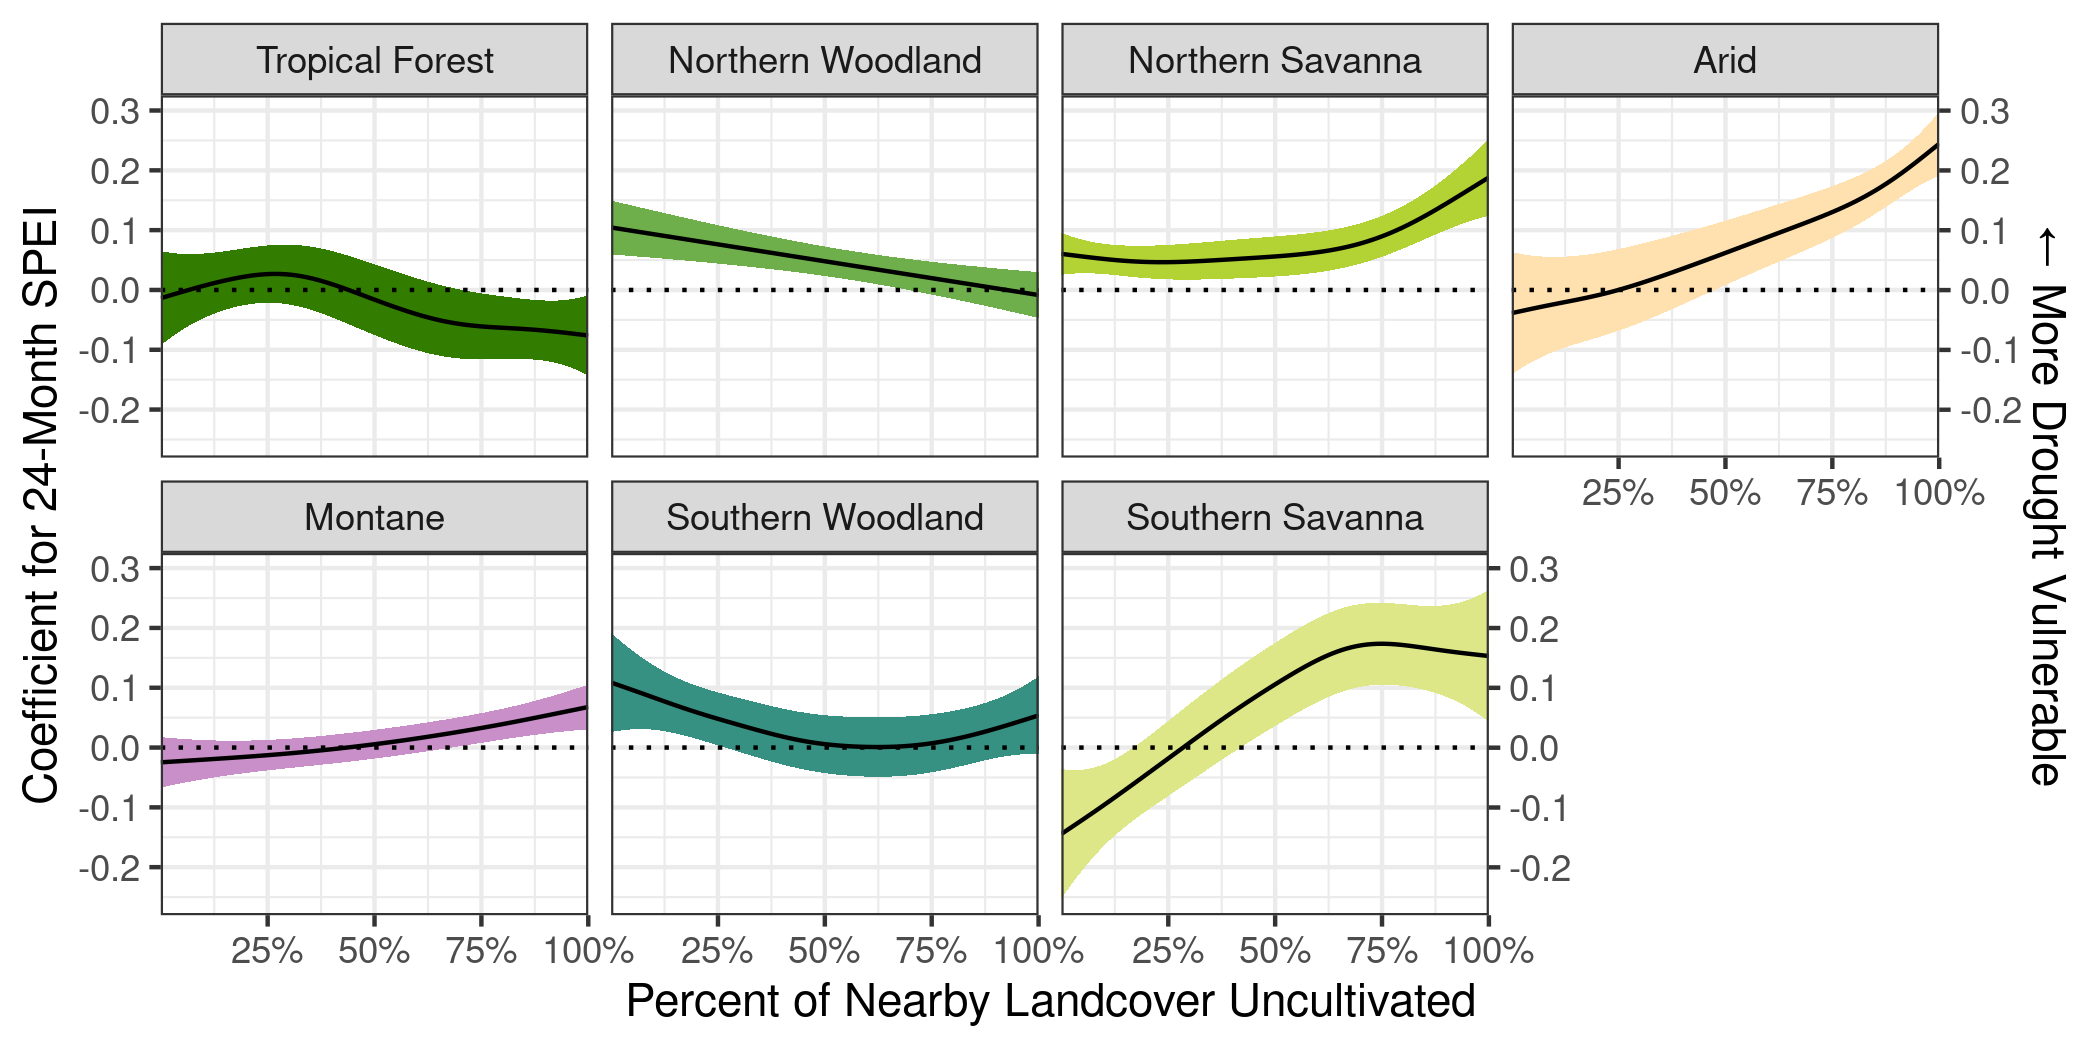
\includegraphics[width=\linewidth]{AEZ_effects_q90.png}
	\end{center}
	\caption{Effect of droughts on child nutrition outcomes by agro-ecological zone (AEZ), varying as a function of the percent of nearby land cover that is uncultivated, estimated with weights censored at the 90th percentile.  Error bands indicate the 95\% confidence interval.}
\end{figure}


\begin{longtable}{l c}
\hline
 & Model 1 \\
\hline
\endfirsthead
\hline
 & Model 1 \\
\hline
\endhead
\hline
\endfoot
\hline
\multicolumn{2}{l}{\scriptsize{$^{***}p<0.001$; $^{**}p<0.01$; $^{*}p<0.05$}}\\
\caption{Parameter estimates for Generalized Additive Model estimating the varying coefficient of SPEI, with CBGPS weights censored at the 90th percentile.}
\label{table:coefficients}
\endlastfoot \\
age                              & $-0.02^{***}$  \\
                                 & $(0.00)$       \\
birth\_order                     & $0.01^{***}$   \\
                                 & $(0.00)$       \\
hhsize                           & $-0.00$        \\
                                 & $(0.00)$       \\
sexFemale                        & $-20.63^{***}$ \\
                                 & $(1.42)$       \\
sexMale                          & $-20.76^{***}$ \\
                                 & $(1.42)$       \\
mother\_years\_ed                & $0.03^{***}$   \\
                                 & $(0.00)$       \\
toiletNo Facility                & $-0.14^{***}$  \\
                                 & $(0.01)$       \\
toiletOther                      & $-0.12^{***}$  \\
                                 & $(0.03)$       \\
toiletPit Latrine                & $-0.11^{***}$  \\
                                 & $(0.01)$       \\
interview\_year                  & $0.01^{***}$   \\
                                 & $(0.00)$       \\
as.factor(calc\_birthmonth)2     & $-0.02$        \\
                                 & $(0.02)$       \\
as.factor(calc\_birthmonth)3     & $0.03^{*}$     \\
                                 & $(0.02)$       \\
as.factor(calc\_birthmonth)4     & $0.03^{*}$     \\
                                 & $(0.02)$       \\
as.factor(calc\_birthmonth)5     & $0.04^{**}$    \\
                                 & $(0.02)$       \\
as.factor(calc\_birthmonth)6     & $0.12^{***}$   \\
                                 & $(0.02)$       \\
as.factor(calc\_birthmonth)7     & $0.09^{***}$   \\
                                 & $(0.02)$       \\
as.factor(calc\_birthmonth)8     & $0.15^{***}$   \\
                                 & $(0.02)$       \\
as.factor(calc\_birthmonth)9     & $0.15^{***}$   \\
                                 & $(0.02)$       \\
as.factor(calc\_birthmonth)10    & $0.21^{***}$   \\
                                 & $(0.02)$       \\
as.factor(calc\_birthmonth)11    & $0.21^{***}$   \\
                                 & $(0.02)$       \\
as.factor(calc\_birthmonth)12    & $0.35^{***}$   \\
                                 & $(0.02)$       \\
head\_age                        & $0.00^{***}$   \\
                                 & $(0.00)$       \\
head\_sexMale                    & $-0.03^{***}$  \\
                                 & $(0.01)$       \\
wealth\_norm                     & $0.50^{***}$   \\
                                 & $(0.02)$       \\
AEZ\_newafr.forest.4             & $-0.09^{**}$   \\
                                 & $(0.03)$       \\
AEZ\_newafr.high.7               & $-0.20^{***}$  \\
                                 & $(0.03)$       \\
AEZ\_newnafr.sav.5               & $0.01$         \\
                                 & $(0.02)$       \\
AEZ\_newnafr.subforest.8         & $0.05$         \\
                                 & $(0.03)$       \\
AEZ\_newsafr.subforest.9         & $0.04$         \\
                                 & $(0.03)$       \\
AEZ\_newseafr.sav.6              & $-0.14^{***}$  \\
                                 & $(0.03)$       \\
EDF: s(latitude,longitude)       & $48.16^{***}$  \\
                                 & $(49.00)$      \\
EDF: s(natural):afr.arid.123     & $3.26^{***}$   \\
                                 & $(3.77)$       \\
EDF: s(natural):afr.forest.4     & $3.32^{*}$     \\
                                 & $(3.88)$       \\
EDF: s(natural):nafr.sav.5       & $3.33^{***}$   \\
                                 & $(3.90)$       \\
EDF: s(natural):seafr.sav.6      & $3.39^{***}$   \\
                                 & $(3.97)$       \\
EDF: s(natural):afr.high.7       & $2.46^{**}$    \\
                                 & $(2.79)$       \\
EDF: s(natural):nafr.subforest.8 & $2.00^{***}$   \\
                                 & $(2.00)$       \\
EDF: s(natural):safr.subforest.9 & $3.32^{*}$     \\
                                 & $(3.89)$       \\
\hline
AIC                              & $833514.31$    \\
BIC                              & $834547.96$    \\
Log Likelihood                   & $-416656.90$   \\
Deviance                         & $31.07$        \\
Deviance explained               & $0.49$         \\
Dispersion                       & $0.00$         \\
R$^2$                            & $0.11$         \\
GCV score                        & $0.00$         \\
Num. obs.                        & $221885$       \\
Num. smooth terms                & $8$            \\
\end{longtable}


\newpage

\section{Model Results With Weights Censored at the 80th Percentile}
\begin{figure}[h!]
	\begin{center}
	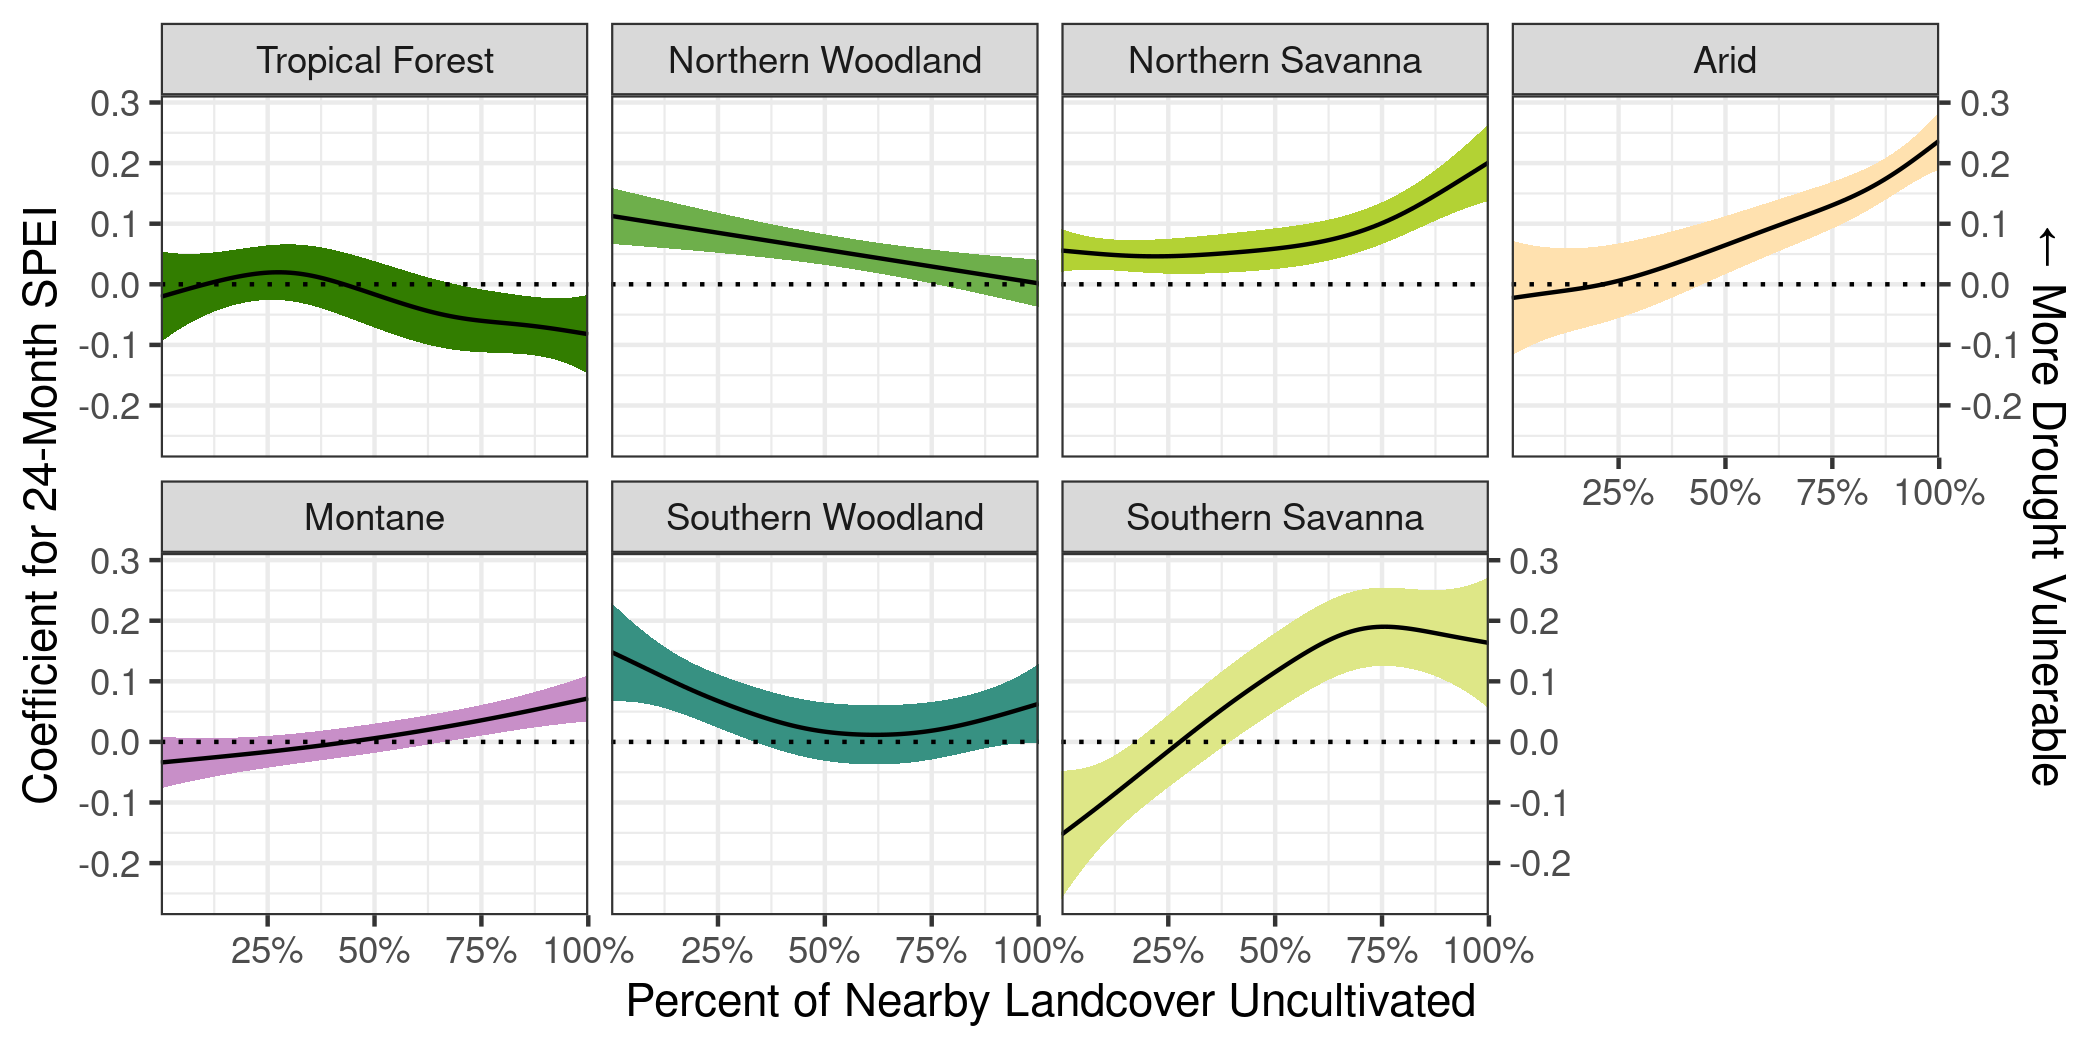
\includegraphics[width=\linewidth]{AEZ_effects_q80.png}
	\end{center}
	\caption{Effect of droughts on child nutrition outcomes by agro-ecological zone (AEZ), varying as a function of the percent of nearby land cover that is uncultivated, estimated with weights censored at the 90th percentile.  Error bands indicate the 95\% confidence interval.}
\end{figure}


\begin{longtable}{l c}
\hline
 & Model 1 \\
\hline
\endfirsthead
\hline
 & Model 1 \\
\hline
\endhead
\hline
\endfoot
\hline
\multicolumn{2}{l}{\scriptsize{$^{***}p<0.001$; $^{**}p<0.01$; $^{*}p<0.05$}}\\
\caption{Parameter estimates for Generalized Additive Model estimating the varying coefficient of SPEI, with CBGPS weights censored at the 80th percentile.}
\label{table:coefficients}
\endlastfoot \\
age                              & $-0.02^{***}$  \\
                                 & $(0.00)$       \\
birth\_order                     & $0.01^{***}$   \\
                                 & $(0.00)$       \\
hhsize                           & $-0.00$        \\
                                 & $(0.00)$       \\
sexFemale                        & $-19.63^{***}$ \\
                                 & $(1.43)$       \\
sexMale                          & $-19.76^{***}$ \\
                                 & $(1.43)$       \\
mother\_years\_ed                & $0.03^{***}$   \\
                                 & $(0.00)$       \\
toiletNo Facility                & $-0.15^{***}$  \\
                                 & $(0.01)$       \\
toiletOther                      & $-0.13^{***}$  \\
                                 & $(0.03)$       \\
toiletPit Latrine                & $-0.12^{***}$  \\
                                 & $(0.01)$       \\
interview\_year                  & $0.01^{***}$   \\
                                 & $(0.00)$       \\
as.factor(calc\_birthmonth)2     & $-0.02$        \\
                                 & $(0.02)$       \\
as.factor(calc\_birthmonth)3     & $0.03^{*}$     \\
                                 & $(0.02)$       \\
as.factor(calc\_birthmonth)4     & $0.03^{*}$     \\
                                 & $(0.02)$       \\
as.factor(calc\_birthmonth)5     & $0.04^{*}$     \\
                                 & $(0.02)$       \\
as.factor(calc\_birthmonth)6     & $0.13^{***}$   \\
                                 & $(0.02)$       \\
as.factor(calc\_birthmonth)7     & $0.10^{***}$   \\
                                 & $(0.02)$       \\
as.factor(calc\_birthmonth)8     & $0.15^{***}$   \\
                                 & $(0.02)$       \\
as.factor(calc\_birthmonth)9     & $0.15^{***}$   \\
                                 & $(0.02)$       \\
as.factor(calc\_birthmonth)10    & $0.22^{***}$   \\
                                 & $(0.02)$       \\
as.factor(calc\_birthmonth)11    & $0.22^{***}$   \\
                                 & $(0.02)$       \\
as.factor(calc\_birthmonth)12    & $0.38^{***}$   \\
                                 & $(0.02)$       \\
head\_age                        & $0.00^{***}$   \\
                                 & $(0.00)$       \\
head\_sexMale                    & $-0.05^{***}$  \\
                                 & $(0.01)$       \\
wealth\_norm                     & $0.51^{***}$   \\
                                 & $(0.02)$       \\
AEZ\_newafr.forest.4             & $-0.10^{**}$   \\
                                 & $(0.03)$       \\
AEZ\_newafr.high.7               & $-0.20^{***}$  \\
                                 & $(0.03)$       \\
AEZ\_newnafr.sav.5               & $0.01$         \\
                                 & $(0.02)$       \\
AEZ\_newnafr.subforest.8         & $0.05$         \\
                                 & $(0.03)$       \\
AEZ\_newsafr.subforest.9         & $0.05$         \\
                                 & $(0.03)$       \\
AEZ\_newseafr.sav.6              & $-0.15^{***}$  \\
                                 & $(0.03)$       \\
EDF: s(latitude,longitude)       & $47.94^{***}$  \\
                                 & $(49.00)$      \\
EDF: s(natural):afr.arid.123     & $3.24^{***}$   \\
                                 & $(3.75)$       \\
EDF: s(natural):afr.forest.4     & $3.24^{*}$     \\
                                 & $(3.78)$       \\
EDF: s(natural):nafr.sav.5       & $3.16^{***}$   \\
                                 & $(3.68)$       \\
EDF: s(natural):seafr.sav.6      & $3.29^{***}$   \\
                                 & $(3.84)$       \\
EDF: s(natural):afr.high.7       & $2.36^{**}$    \\
                                 & $(2.64)$       \\
EDF: s(natural):nafr.subforest.8 & $2.00^{***}$   \\
                                 & $(2.00)$       \\
EDF: s(natural):safr.subforest.9 & $3.16^{***}$   \\
                                 & $(3.69)$       \\
\hline
AIC                              & $842174.38$    \\
BIC                              & $843199.14$    \\
Log Likelihood                   & $-420987.79$   \\
Deviance                         & $24.27$        \\
Deviance explained               & $0.49$         \\
Dispersion                       & $0.00$         \\
R$^2$                            & $0.11$         \\
GCV score                        & $0.00$         \\
Num. obs.                        & $221885$       \\
Num. smooth terms                & $8$            \\
\end{longtable}


\end{document}
